\documentclass[14pt, a4paper]{extreport}

% increase toc depth up to subsubsection
\setcounter{tocdepth}{3}
\setcounter{secnumdepth}{3}

\usepackage{tabu}
\usepackage{color}
\usepackage{array}
\usepackage{epstopdf}
\usepackage[russian]{babel}
\usepackage[utf8x, utf8]{inputenc}
\usepackage{tikz}
\usetikzlibrary{positioning, shapes.misc, shapes.geometric, arrows, shapes.multipart, shapes.arrows}
\usepackage{pgfplots}
\usepgfplotslibrary{dateplot}
\usepackage{amsmath}
\usepackage{algorithm2e}
\usepackage{algorithmic}
\usepackage{xcolor, colortbl}
\usepackage{mdframed}
\usepackage{textcase}
\usepackage{tabularx}
\usepackage[T2A,T1]{fontenc}
% 
\usepackage{indentfirst}
\usepackage{listings}
\lstset{breaklines=true}
% setup  page fields
\usepackage{geometry}
\geometry{left=25mm}
\geometry{right=20mm}
\geometry{top=20mm}
\geometry{bottom=20mm}
% set line interval
\usepackage{setspace}
\onehalfspacing
% set footnotesize to 12 pt (for normalsize equal to 14 pt)
\renewcommand{\footnotesize}{\small}

\usepackage{titlesec}
\titleformat{\chapter}{\filcenter\bfseries}{\thechapter.}{1em}{}
\titleformat{\section}{\filcenter\bfseries}{\thesection}{1em}{}
\titleformat{\subsection}{\filcenter\bfseries}{\thesubsection}{1em}{}
\titleformat{\subsubsection}{\filcenter\bfseries}{\thesubsubsection}{1em}{}
\titleformat{\paragraph}{\filcenter\bfseries}{\paragraph}{1em}{}
\titlespacing*{\chapter}{0pt}{10pt}{10pt}

% make page number in top right corner
\usepackage{fancyhdr}
% rename abstract
\AtBeginDocument{\addto\captionsenglish{\def\abstractname{\MakeTextUppercase{Реферат}}}}
% counters
\usepackage[figure, table, page, enumiv]{totalcount}
%
\addto\captionsrussian
{
  \renewcommand{\contentsname}
    {\hfill{\normalsize\MakeTextUppercase{Содержание}}\hfill}
}
%
\addto\captionsrussian
{
  \renewcommand{\bibname}{\hfill\normalsize\MakeTextUppercase{Список использованных источников}\hfill}
}

\usepackage{tocloft}
% add dots for chapters
\renewcommand{\cftchapleader}{\cftdotfill{\cftdotsep}}
\renewcommand\cftchapfont{\mdseries}
\renewcommand\cftchappagefont{\mdseries}
% add dot after chapter number
\renewcommand{\cftchapaftersnum}{.}
%
\usepackage{caption}
\usepackage{subcaption}
\captionsetup[figure]{labelsep=space}
\captionsetup[table]{labelsep=space}

\usepackage{etoolbox}
\makeatletter
\patchcmd{\chapter}{\if@openright\cleardoublepage\else\clearpage\fi}{}{}{}
\makeatother

%
% flow chart commands
\tikzstyle{startstop} = [rectangle, rounded corners, minimum width=3cm, minimum height=0.5cm, text centered, draw=black, fill=red!30]
\tikzstyle{process} = [rectangle, minimum width=3cm, minimum height=0.5cm, text centered, draw=black, fill=orange!30]
\tikzstyle{decision} = [diamond, aspect=2, minimum width=1mm, minimum height=1mm, text centered, draw=black, fill=green!30]
\tikzstyle{arrow} = [thick,->,>=stealth]
%

% declare new operator for correct \limits usage
\DeclareMathOperator*{\argmin}{arg\,min}

\title{}
\date{}

\begin{document}
\RestyleAlgo{boxruled}
% style for top right corner page number
\fancypagestyle{plain}{%
    \fancyhf{} % clear all header and footer fields
    \fancyhead[R]{\thepage} % except the right top corner
    \renewcommand{\headrulewidth}{0pt} % remove line between header and main text
}
\pagestyle{plain}

\renewcommand\abstractname{\MakeTextUppercase{Реферат}}

\begin{titlepage}

\newcommand{\StudentName}{Данилычев Иван}
\newcommand{\Group}{1O-106М}
\newcommand{\CourseName}{Информационный поиск}
\newcommand{\LabNum}{1}
\newcommand{\Subject}{Поиск по постам сообществ ВКонтакте}
\newcommand{\PrepName}{Калинин А.\,Л.}

\newpage

\begin{center}
Московский Авиационный Институт \\*
(национальный исследовательский университет) \\*
Факультет прикладной математики и физики \\*
\hrulefill
\end{center}

\begin{center}
Кафедра вычислительной математики и программирования
\end{center}

\vspace{6em}

\begin{center}
\Large \CourseName \\
	Курсовой проект \\
  <<\Subject>>
\end{center}

\vspace{2em}
\vspace{6em}

\begin{flushright}
	\StudentName, \\
	группа: \Group \\
\vspace{1em}
руководитель:\\
   \PrepName \\
\end{flushright}

\vspace{\fill}

\begin{center}
Москва, 2016
\end{center}

\end{titlepage}


\newpage
\vspace*{-25mm}
\tableofcontents
\newpage

% Examples:
%\addcontentsline{toc}{section}{Заголовок}
%\section*{Заголовок}

%\addcontentsline{toc}{section}{Введение}
%\section{Введение}
\chapter{\MakeTextUppercase{Веб-интерфейс}}
Для фронтенда был выбран фреймворк Flask~\cite{flask}, написанный на Python, поскольку у меня уже был опыт работы с ним. Возможно, стоило воспользоваться более быстрым, и тем более --- асинхронным решением, например, vibe.d (язык D), но на его изучение ушло бы больше времени.

Фронтенд состоит из двух страниц:
\begin{itemize}
  \item Заглавная страница с логотипом и полем ввода запроса;
  \item Страница с поисковой выдачей.
\end{itemize}

\begin{figure}[!htb]
  \centering
  
\includegraphics[scale=0.55]{pics/frontend.png}
  \caption{Заглавная страница}
  \label{fig:frontend}
\end{figure}

\begin{figure}[!htb]
  \centering
  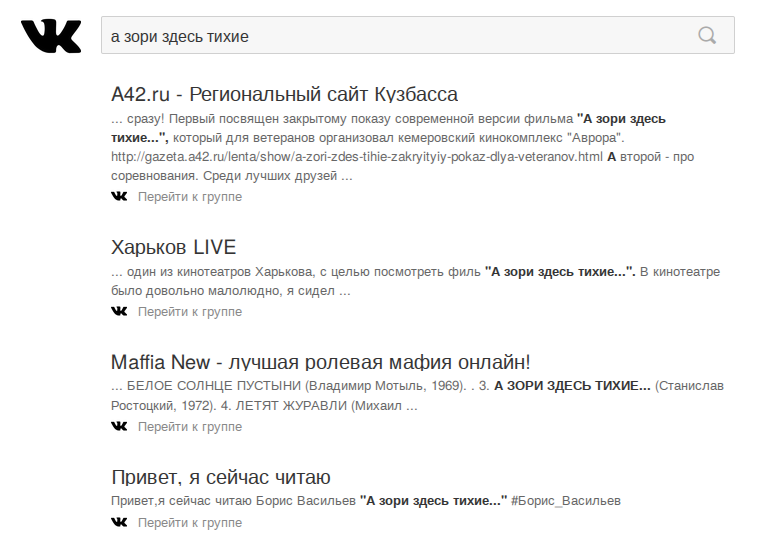
\includegraphics[scale=0.45]{pics/results.png}
  \caption{Поисковая выдача}
  \label{fig:results}
\end{figure}

Поскольку исходные документы --- сообщения на стенах групп --- нигде на сервере не хранятся, при каждом новом запросе их приходится скачивать через API ВКонтакте, который, к счастью, не накладывает на эту операцию никаких ограничений. Скачанные документы передаются клиенту и обрабатываются партиями по 10 штук при каждом клике по кнопке <<Ещё>>, что позволяет существенно снизить ощущаемое клиентом время задержки (в которое вносит свой вклад и ВКонтакте).


\chapter{\MakeTextUppercase{Построение сниппетов}}

Большинство постов ВКонтакте достаточно коротки и оказываются в выдаче целиком, поэтому было принято решение, что для данного проекта достаточно:
\begin{itemize}
  \item Подсветить все ключевые слова в посте;
  \item Включить в выдачу все слова в окне ширины $d$ вокруг ключевых, а пропуски заполнить многоточиями;
  \item При необходимости --- обрезать текст до $n$ символов.
\end{itemize}

Код на Python:

\begin{lstlisting}
  def make_snippet(text, terms, dist, max_length):
    # eliminate <br> and get list of words
    single_line = linebreak_killer.sub(' ', text)
    split_text = single_line.split(' ')

    punct_split = lambda x: (''.join([ch.upper() if ch not in punctuation_marks else ' ' for ch in x])).split(' ')

    # whether a token or list of tokens starts with a normalized search term
    swc = lambda token, term: token.startswith(term) and sum(map(lambda l: l[0] == l[1], zip(token, term))) >= len(token) / 2.
    checker = lambda i, term: any([swc(t, term) for t in tokens[i]]) if isinstance(tokens[i], list) else swc(tokens[i], term)

    # find all words we need to highlight
    tokens = map(punct_split, split_text)
    shallow_occurences = [[i for i in xrange(len(tokens)) if checker(i, term)] for term in terms]
    occurences = sorted(list(itertools.chain(*shallow_occurences)))

    if not occurences:
        return text

    highlighted_text = map(lambda i: \
        '<b>%s</b>' % split_text[i] if i in occurences else split_text[i], \
        range(len(split_text))
    )
    result_tmp = []

    # build occurences list
    for i in xrange(len(occurences)):
        d = dist if i in [0, len(occurences)-1] else dist / 2
        result_tmp.append((max(0, occurences[i] - d), min(occurences[i] + d, len(highlighted_text))))

    # merge adjacent occurences, if necessary
    final_result = []
    for occ in result_tmp:
        if not final_result or occ[0] > final_result[-1][1]:
            final_result.append([occ[0], occ[1]])
        else:
            final_result[-1][1] = occ[1]

    joiner = lambda l: ' '.join(l)
    separator = ' ... '

    snippet_string = separator.join(map(joiner, [highlighted_text[occ[0]:occ[1]] for occ in final_result]))
    head = separator if final_result[0][0] > 0 else ''
    tail = separator if final_result[-1][1] < len(highlighted_text) else ''

    return head + snippet_string + tail
\end{lstlisting}

\newpage
\clearpage
%
\addcontentsline{toc}{chapter}{\MakeTextUppercase{Список использованных источников}}
\begin{thebibliography}{}
\bibitem{flask} http://flask.pocoo.org
\end{thebibliography}

\end{document}
